\documentclass[11pt]{article}

%\usepackage{times}
\usepackage{fullpage}



% For figures
\usepackage{graphicx}
\usepackage{subfigure}

% For citations
%\usepackage{natbib}

% For algorithms
\usepackage{algorithm}
\usepackage{algorithmic}

\usepackage[colorlinks=true]{hyperref}

% Packages hyperref and algorithmic misbehave sometimes.  We can fix
% this with the following command.
\newcommand{\theHalgorithm}{\arabic{algorithm}}

% other packages
\usepackage{amsthm}
\usepackage{Definitions}
\usepackage{pdfsync}
\usepackage{color}
\usepackage{xspace}
\newcommand{\Note}[1]{{\color{red}{\bf\sf [note: #1]}}}
\usepackage{enumitem}

\newtheorem{claim}{Claim}

\newcommand{\littleheader}[1]{\noindent \textbf{#1} }
\newenvironment{proofsketch}{\par\noindent{\bfseries\upshape Proof Sketch:}}{\hfill \qed}

\newcommand{\R}{\mathbb{R}}

% graph notations
\newcommand{\Graph}{\Gcal}
\newcommand{\Node}{\Vcal}
\newcommand{\nNode}{n}
\newcommand{\Edge}{\Ecal}
\newcommand{\nEdge}{m}
\newcommand{\Item}{\Lcal}
\newcommand{\nItem}{\ell}
\newcommand{\Ground}{\Zcal}
\newcommand{\nGround}{N}
\newcommand{\Ind}{\Ical}

% constraints
\newcommand{\budget}{b}
\newcommand{\attention}{u}

% solution
\newcommand{\Greedy}{G}
\newcommand{\g}{g}
\newcommand{\Optimal}{O}
\newcommand{\OPT}{\mathrm{OPT}}

\newcommand{\spn}{\mathrm{sp}}
\newcommand{\cur}{c}


\newcommand{\continmax}{\textsc{ConTinEst}\xspace}
\newcommand{\budgetmax}{\textsc{BudgetMax}\xspace}
\newcommand{\gdegree}{{GreedyDegree}\xspace}
\newcommand{\rmnum}[1]{\romannumeral #1}
\newcommand{\netrate}{\textsc{NetRate}\xspace}

% yichen
\newcommand{\X}{\mathcal{X}}

\title{When LSTM Meets Point Process : \\ Predicting Context-Sensitive Activities}

\author{Nan Du
}

\date{}

\begin{document}

\maketitle

%\begin{abstract}
%	
%\end{abstract}

\section{Problem description and background}

User activities often arise as sequences of events along time. For instance, users might go to work, airports, gas stations, parks, cinemas, church, restaurants, groceries at different time and days in a week. They might listen to different albums, watch different videos, and even catch different diseases as time changes. Accurately predicting the next activity at the right moment will have potential applications of great significance. For mainstream personal assistants, like Google Now shown in Figure~\ref{demo}, because people tend to visit different places dependent on the temporal/spatial contexts like morning vs. evening, weekdays vs. weekend, successfully predicting the next places that users will visit at the most likely time will make such services more relevant and usable. Furthermore, for modern healthcare, patients may have several diseases that have complicated dependencies on each other. The occurrence of one disease can trigger the progression of others. Accurately estimating when a probable disease might occur can effectively help to take proactive steps to reduce the potential risks in the future. 

\begin{figure*}[h!]
\centering
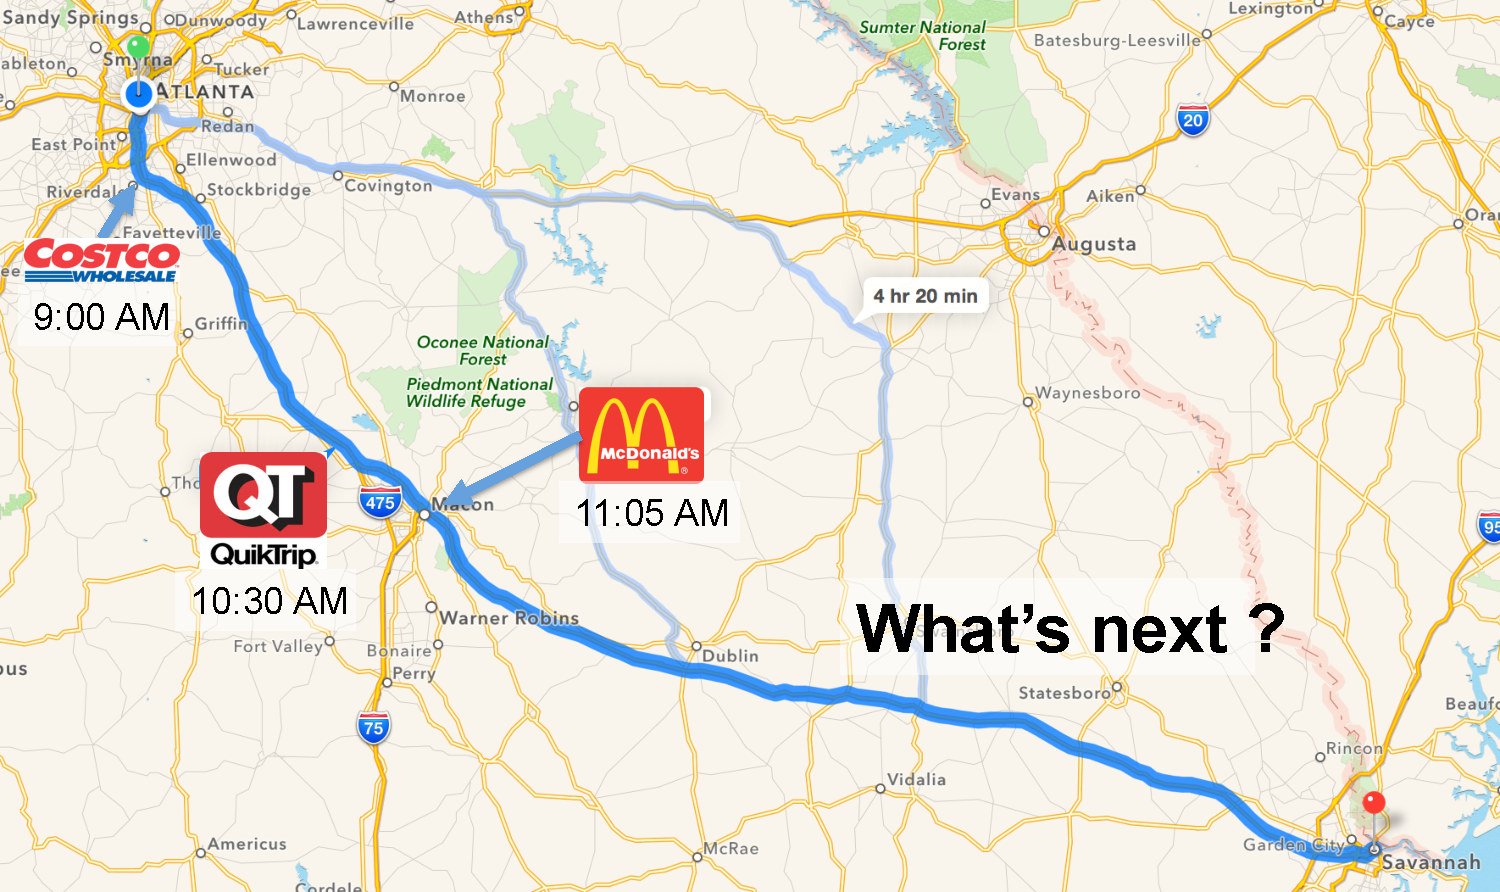
\includegraphics[width=0.55\textwidth]{fig1}
\caption{\label{demo}Given the sequence of past visited places, can we predict where the user will go next at what time ?}
\end{figure*}

More recently, recurrent neural networks with long short-term memory (LSTM) architecture are reported to be able to perform as well as existing well-developed systems in sequence modeling tasks, such as machine translation~\cite{SutVinLe2014}, speech recognition~\cite{SakSenBea2014}, etc. On the other hand, point processes~\cite{CoxIsh1980}, are good at capturing inter-event time intervals among asynchronous activities and events. 

The key idea of this project is to have the LSTM model the diversity of event types (\eg, places, diseases) while the point process captures the inter-event time duration based on the sequence of past events, accordingly. 

\section{Dataset}
\begin{itemize}
	\item \textbf{last.fm}\footnote{\url{http://www.dtic.upf.edu/\~{}ocelma/MusicRecommendationDataset/lastfm-1K.html}} consists of the music listening histories of around 1,000 users over 3,000 different albums. There are around 20,000 user-album pairs with more than one million events.
	\item \textbf{tmall.com} \footnote{\url{http://ijcai-15.org/index.php/repeat-buyers-prediction-competition}} contains online shopping records. There are around 100K events between 26,376 users and 2,563 stores.
	\item \textbf{MIMIC II} (Multiparameter Intelligent Monitoring in Intensive Care II) is a medical dataset that is a collection of de-identified clinical visit records of Intensive Care Unit patients between 2001 and 2008 from a single tertiary teaching hospital. We have filtered out 650 patients and 204 diseases. For a given pair of patient and disease, each event corresponds to the visiting time when this patient was diagnosed to have the respective disease.
\end{itemize}

\section{Technical Steps}

The output from the LSTM layer corresponds to a new representation for the current input label given the sequence of past labels so far. We assume that the conditional distribution for the time interval up to the next event conforms to a Weibull distribution where the scaling parameter is a nonlinear function of such output from the LSTM layer. We can put a softmax layer above the LSTM layer with a cross-entropy loss for the sequence modeling task while maximizing the log-likelihood of observing this whole sequence of events so far. We can iteratively optimize with respect to these two objective functions to learn the parameters, respectively. 


%KapSubKarSriJaiSch15

\bibliographystyle{abbrv}

\bibliography{bibfile}

\end{document}
